\documentclass[12pt,fleqn]{article}
\usepackage{vkCourseML}
\usepackage{cancel}
%\usepackage{vkCourseML}
\hypersetup{unicode=true}
%\usepackage[a4paper]{geometry}
\usepackage[hyphenbreaks]{breakurl}
\usepackage{graphicx}
\usepackage{float}        % для [H]
\graphicspath{{./images/}}% папка с картинками
\theorembodyfont{\rmfamily}
\newtheorem{esProblem}{Задача}

\begin{document}

\title{Машинное обучение, ФКН ВШЭ\\Семинар №5}

\author{}
\date{}

\maketitle

\section*{AUC-ROC}
На лекции мы познакомились с такой важной метрикой качества бинарной классификации, как площадь под ROC-кривой (AUC-ROC). Напомним её определение. Рассмотрим задачу бинарной классификации с метками классов $\mathbb{Y}=\{-1,+1\}$, и пусть задан некоторый алгоритм $b(x)$, позволяющий вычислять оценку принадлежности объекта $x$ положительному классу. AUC-ROC позволяет оценивать качество классификации для семейства алгоритмов следующего вида:

$$
a(x ; t)=\left\{\begin{array}{l}
-1, b(x) \leq t \\
+1, b(x)>t
\end{array}\right.
$$

т.е. алгоритмов, присваивающих метки объектам в соответствии с оценками $b(x)$, отсекая их по некоторому порогу $t$. Каждый алгоритм (получающийся при фиксации значения порога $t$ ) представляется точкой на плоскости (FPR, TPR), где

$$
\begin{aligned}
& \mathrm{FPR}=\frac{\mathrm{FP}}{\mathrm{FP}+\mathrm{TN}}=\frac{\mathrm{FP}}{\ell_{-}} \\
& \mathrm{TPR}=\frac{\mathrm{TP}}{\mathrm{TP}+\mathrm{FN}}=\frac{\mathrm{TP}}{\ell_{+}}
\end{aligned}
$$

$\ell_{-}, \ell_{+}$- количество объектов отрицательного и положительного классов соответственно. AUC-ROC, в свою очередь, является площадью под получившейся кривой.



Изучим подробнее некоторые важные свойства данной метрики. \\


Критерий AUC-ROC имеет большое число интерпретаций - например, он равен вероятности того, что случайно выбранный положительный объект окажется позже случайно выбранного отрицательного объекта в ранжированном списке, порожденном $b(x)$. Разберем подробнее немного другую формулировку.  \\


\textbf{Задача 1.1.} В ранжировании часто используется функционал «доля дефектных пар». Его можно определить и для задачи бинарной классификации.

Пусть дан классификатор $b(x)$, который возвращает оценки принадлежности объектов классу +1 , и пусть все значения $b\left(x_{i}\right), i=\overline{1, \ell}$, для некоторой выборки $X=\left\{\left(x_{i}, y_{i}\right)\right\}_{i=1}^{\ell}$ различны. Отсортируем все объекты по возрастанию ответа классификатора: $b\left(x_{(1)}\right)<\cdots<b\left(x_{(\ell)}\right)$. Обозначим истинные ответы на этих объектах

через $y_{(1)}, \ldots, y_{(\ell)}$. Тогда доля дефектных пар записывается как

$$
D P(b, X)=\frac{2}{\ell(\ell-1)} \sum_{i<j}^{\ell}\left[y_{(i)}>y_{(j)}\right] .
$$

Как данный функционал связан с AUC-ROC? \\


	\begin{esSolution}
	Для начала разберем процедуру построения ROC-кривой. Сперва все объекты сортируются по неубыванию оценки $b(x)$, тем самым формируя список $x_{(1)}, \dots, x_{(\ell)}.$ Заметим, что для построения ROC-кривой достаточно рассмотреть\\ $(\ell+1)$ различных значений порога $t$, соответствующих всем различным способам классификации выборки, порожденным алгоритмом $b(x)$,~--- например, в качестве таких порогов можно рассмотреть следующий набор:
	\begin{align*}
		\hspace*{-5cm}&t_\ell = b(x_{(\ell)}) + 1,\\
		&t_i = \frac{b(x_{(i)}) + b(x_{(i+1)})}{2} , \, i = \overline{1, \ell -1},\\
		&t_0 = b(x_{(1)}) - 1.
	\end{align*}	
	Зафиксируем значение порога $t = t_\ell =  b(x_{(\ell)}) + 1$, в этом случае имеем
	$$\text{FPR} = \frac{\text{FP}}{\ell_-} = \frac{0}{\ell_-} = 0,$$
	$$\text{TPR} = \frac{\text{TP}}{\ell_+} = \frac{0}{\ell_+} = 0.$$
	Таким образом, алгоритму $a(x; t_\ell)$ соответствует точка (0; 0) на плоскости, откуда начинается построение ROC-кривой.
		 Будем перебирать пороги в порядке невозрастания их значения, начиная с $t_{\ell}$. Пусть мы хотим уменьшить значение порога с $t_i$ до $t_{i-1}$. При этом классификация объекта $x_{(i)}$ (и только его) изменится с отрицательной на положительную. Рассмотрим 2 случая.
	
        \begin{figure}[H]
          \centering
          \includegraphics[width=0.8\linewidth]{2025_10_04_c092876edd6a5f417b07g-2.jpg}
          \label{fig:roc-procedure}
        \end{figure}


	\begin{enumerate}
		\item $y_{(i)} = +1.$ В этом случае классификатор начнет верно классифицировать объект, на котором ранее допускал ошибку, при этом FPR не изменится, а TPR повысится на~$\frac{1}{\ell_+}.$
		\item $y_{(i)} = -1.$ В этом случае классификатор начнет ошибаться на объекте, который ранее классифицировал верно, при этом TPR не изменится, а FPR повысится на  $\frac{1}{\ell_-}.$
	
	\end{enumerate}
	
        \begin{figure}[H]
          \centering
          \includegraphics[width=0.6\linewidth]{2025_10_04_c092876edd6a5f417b07g-3.jpg}
          \label{fig:roc-step}
        \end{figure}
	
	Теперь рассмотрим, как при этом изменяется AUC-ROC. Заметим, что область под ROC-кривой состоит из непересекающихся прямоугольников, каждый из которых снизу ограничен осью FPR, а сверху~--- одним из горизонтальных отрезков, соответствующих второму из рассмотренных случаев. Поэтому каждый раз, когда имеет место второй случай, к текущей накопленной площади под кривой (которая изначально в точке (0; 0) равна 0) добавляется площадь прямоугольника, горизонтальные стороны которого равны $\frac{1}{\ell_-}$, а вертикальные равны $\frac{1}{\ell_+} \sum_{j=i+1}^{\ell} [y_{(j)} = +1]$ (доля уже рассмотренных положительных объектов среди всех положительных), поэтому в этом случае текущее значение AUC-ROC увеличивается на $\frac{1}{\ell_- \ell_+} \sum_{j=i+1}^\ell [y_{(j)} = +1].$
	Итого, финальное значение AUC-ROC можно посчитать~следующим образом:
       \begin{align*}
      \text{AUC} &= \frac{1}{\ell_{+} \ell_{-}} \sum_{i = 1}^{\ell} [y_{(i)} = -1] \sum_{j = i + 1}^{\ell} [y_{(j)} = +1] =\\
       &= \frac{1}{\ell_{+} \ell_{-}}
        \sum_{i = 1}^{\ell} \sum_{j = i + 1}^{\ell} [y_{(i)} < y_{(j)}] =\\
        &= \frac{1}{\ell_{+} \ell_{-}} \sum_{i < j}^{\ell} (1 - [y_{(i)} = y_{(j)}] - [y_{(i)} > y_{(j)}]) =\\
        &= \frac{1}{\ell_{+} \ell_{-}} \sum_{i < j}^{\ell} (1 - [y_{(i)} = y_{(j)}]) - \frac{1}{\ell_{+} \ell_{-}} \sum_{i < j}^{\ell} [y_{(i)} > y_{(j)}] =\\
        &= \frac{1}{\ell_{+} \ell_{-}} \sum_{i < j}^{\ell} ([y_{(i)} \ne y_{(j)}]) - \frac{1}{\ell_{+} \ell_{-}} \sum_{i < j}^{\ell} [y_{(i)} > y_{(j)}] =\\
        &=
        \frac{\ell_{+} \ell_{-}}{\ell_{+} \ell_{-}}
        - \frac{1}{\ell_{+} \ell_{-}}
        \sum_{i < j}^{\ell}
        [y_{(i)} > y_{(j)}]
        = 1
        -
        \frac{1}{\ell_{+} \ell_{-}}
        \sum_{i < j}
        [y_{(i)} > y_{(j)}].
\end{align*}

	Отсюда получаем, что AUC-ROC и доля дефектных пар связаны следующим соотношением:
	$$\text{DP}(b, X) = \frac{2 \ell_- \ell_+}{\ell (\ell -1)} (1 - \text{AUC} (b, X))).$$

Заметим, что в случае, когда несколько объектов выборки имеют равные значения $b(x)$, при уменьшении значения порога с $t_i > b(x)$  до $t_{i-1} < b(x),$ где $x$ — один из таких объектов, изменение значений FPR и TPR происходит одновременно, поэтому  соответствующий участок ROC-кривой будет наклонным, а не горизонтальным или вертикальным. \\
	

\textbf{Задача 1.2.} Пусть даны выборка $X$, состоящая из 5 объектов, и классификатор $b(x)$, предсказывающий оценку принадлежности объекта положительному классу. Предсказания $b(x)$ и реальные метки объектов приведены ниже:

$$
\begin{array}{ll}
b\left(x_{1}\right)=0.2, & y_{1}=-1, \\
b\left(x_{2}\right)=0.4, & y_{2}=+1, \\
b\left(x_{3}\right)=0.1, & y_{3}=-1, \\
b\left(x_{4}\right)=0.7, & y_{4}=+1, \\
b\left(x_{5}\right)=0.05, & y_{5}=+1 .
\end{array}
$$

Вычислите $A U C$ - $R O C$ и $P R - ROC$ для b(x) на выборке $X$.  \\

	\begin{esSolution}
		В соответствии с процессом построения ROC-кривой, описанным в предыдущей задаче, отсортируем оценки $b(x_i)$ в порядке их неубывания: $(b(x_{(i)}))_{i=1}^\ell = (0.05, 0.1, 0.2, 0.4, 0.7)$. Также составим последовательность реальных меток объектов из этого упорядоченного списка: $(y_{(i)})_{i=1}^\ell = (+1, -1, -1, +1, +1)$.
		
		Построим ROC-кривую (см. рис.~\ref{problem}), откуда $\text{AUC-ROC} = \frac{2}{3}$.

	\begin{figure}[h]
		\center{\includegraphics[width=0.6\linewidth]{2025_10_04_c092876edd6a5f417b07g-4.jpg}
		\caption{Иллюстрация к задаче 1.2.}
		\label{problem}
	\end{figure}
	
Заметим, что при вычислении AUC-ROC на некоторой выборке $X$ для итогового классификатора $a(x; t)$ важны не конкретные значения $b(x_i), \, i = \overline{1, \ell},$ а порядок расположения объектов в отсортированном по неубыванию списке $b(x_{(1)}), \dots, b(x_{(\ell)}),$ порожденным алгоритмом $b(x)$. Таким образом, для фиксированной выборки $X$ алгоритм $b(x)$ задаёт перестановку на её объектах, которая в дальнейшем используется при расчёте AUC-ROC. \\
    

\textbf{Задача 1.3.} Пусть $b(x)$ - некоторый классификатор, предсказывающий оценку принадлежности объекта $x$ положительному классу, и при этом AUC-ROC множества классификаторов $a(x ; t)$, порожденных $b(x)$, на некоторой выборке $X$ принимает значение, меньшее 0.5. Как можно скорректировать прогнозы классификаторов $a(x ; t)$, чтобы они были более осмысленными по сравнению с прогнозами классификатора, выдающего случайные ответы? \\
  
\begin{esSolution}
Для некоторого классификатора $a(x;t)$ рассмотрим классификатор $a^*(x;t)$, выдающий противоположные метки по сравнению с $a(x;t)$, т.е.:
		$$a^*(x;t) = -a(x;t).$$
		При этом TP и FP на обучающей выборке для некоторого классификатора $a^*(x;t)$ будут принимать следующие значения:
		\begin{align*}
			\text{TP}(a^*(x; t), X) = 
			\sum_{i=1}^\ell [y_i = +1]&[a^*(x;t) = +1] =\\
			&= \sum_{i=1}^\ell [y_i = +1][a(x;t) = -1] = 
			\text{FN}(a(x; t), X),\\
			\text{FP}(a^*(x; t), X) = 
			\sum_{i=1}^\ell [y_i = -1]&[a^*(x;t) = +1] =\\
			&=\sum_{i=1}^\ell [y_i = -1][a(x;t) = -1] = \text{TN}(a(x; t), X).			
		\end{align*}
		Отсюда имеем
		\begin{align*}
			\text{TPR}(a^*(x;t), X) = 
			\frac{\text{TP}(a^*(x;t), X)}{\ell_+} &= 
			\frac{\text{FN}(a(x;t), X)}{\ell_+} =\\
			&=\frac{\ell_+ - \text{TP}(a(x;t), X)}{\ell_+} 
			= 1 - \text{TPR}(a(x;t), X),\\
			\text{FPR}(a^*(x;t), X) = 
			\frac{\text{FP}(a^*(x;t), X)}{\ell_-} &= 
			\frac{\text{TN}(a(x;t), X)}{\ell_-} =\\
			&=\frac{\ell_- - \text{FP}(a(x;t), X)}{\ell_-} 
			= 1 - \text{FPR}(a(x;t), X),			
		\end{align*}
		поэтому классификатор $a^*(x;t)$ будет представлен на плоскости точкой, симметричной точке, отвечающей классификатору $a(x;t)$, относительно точки~$\left(0.5; 0.5 \right)$. 
		
		Рассмотрим ROC-кривую для множества классификаторов~$a(x;t).$ Пусть площадь областей единичного квадрата, находящихся между его диагональю и частями ROC-кривой, расположенных под ней, равна~$S_-,$ а между диагональю и частями ROC-кривой, расположенных над диагональю,~"---~$S_+.$ Тогда AUC-ROC для такой кривой принимает значение $0.5 + S_+ - S_- < 0.5$ (по условию), отсюда~$S_+ - S_- < 0.$
		
		Как было показано ранее, ROC-кривая для множества классификаторов~$a^*(x;t)$ симметрична ROC-кривой для множества классификаторов~$a(x;t),$ а потому для первой кривой область, соответствующая площади~$S_-,$ будет расположена над диагональю единичного квадрата, площади~$S_+$ "--- под диагональю. Отсюда AUC-ROC для множества классификаторов~$a^*(x;t)$ будет принимать значение $0.5 - S_+ + S_- > 0.5,$ а потому прогнозы классификаторов из этого множества  более осмысленны по сравнению со случайным классификатором. \\

\textbf{Задача 1.4.} На ответах алгоритма b(x), отнормированных на интервал от 0 до 1,
объекты отрицательного класса распределены с плотностью $ p(b) = 2 − 2 b$, а объекты
положительного класса распределены с плотностью p(b) = 2b см. рис. \ref{fig:densities}). Выпишите
формулу для ROC-кривой и посчитайте площадь под ней.

\begin{figure}[th!]
	\centering
	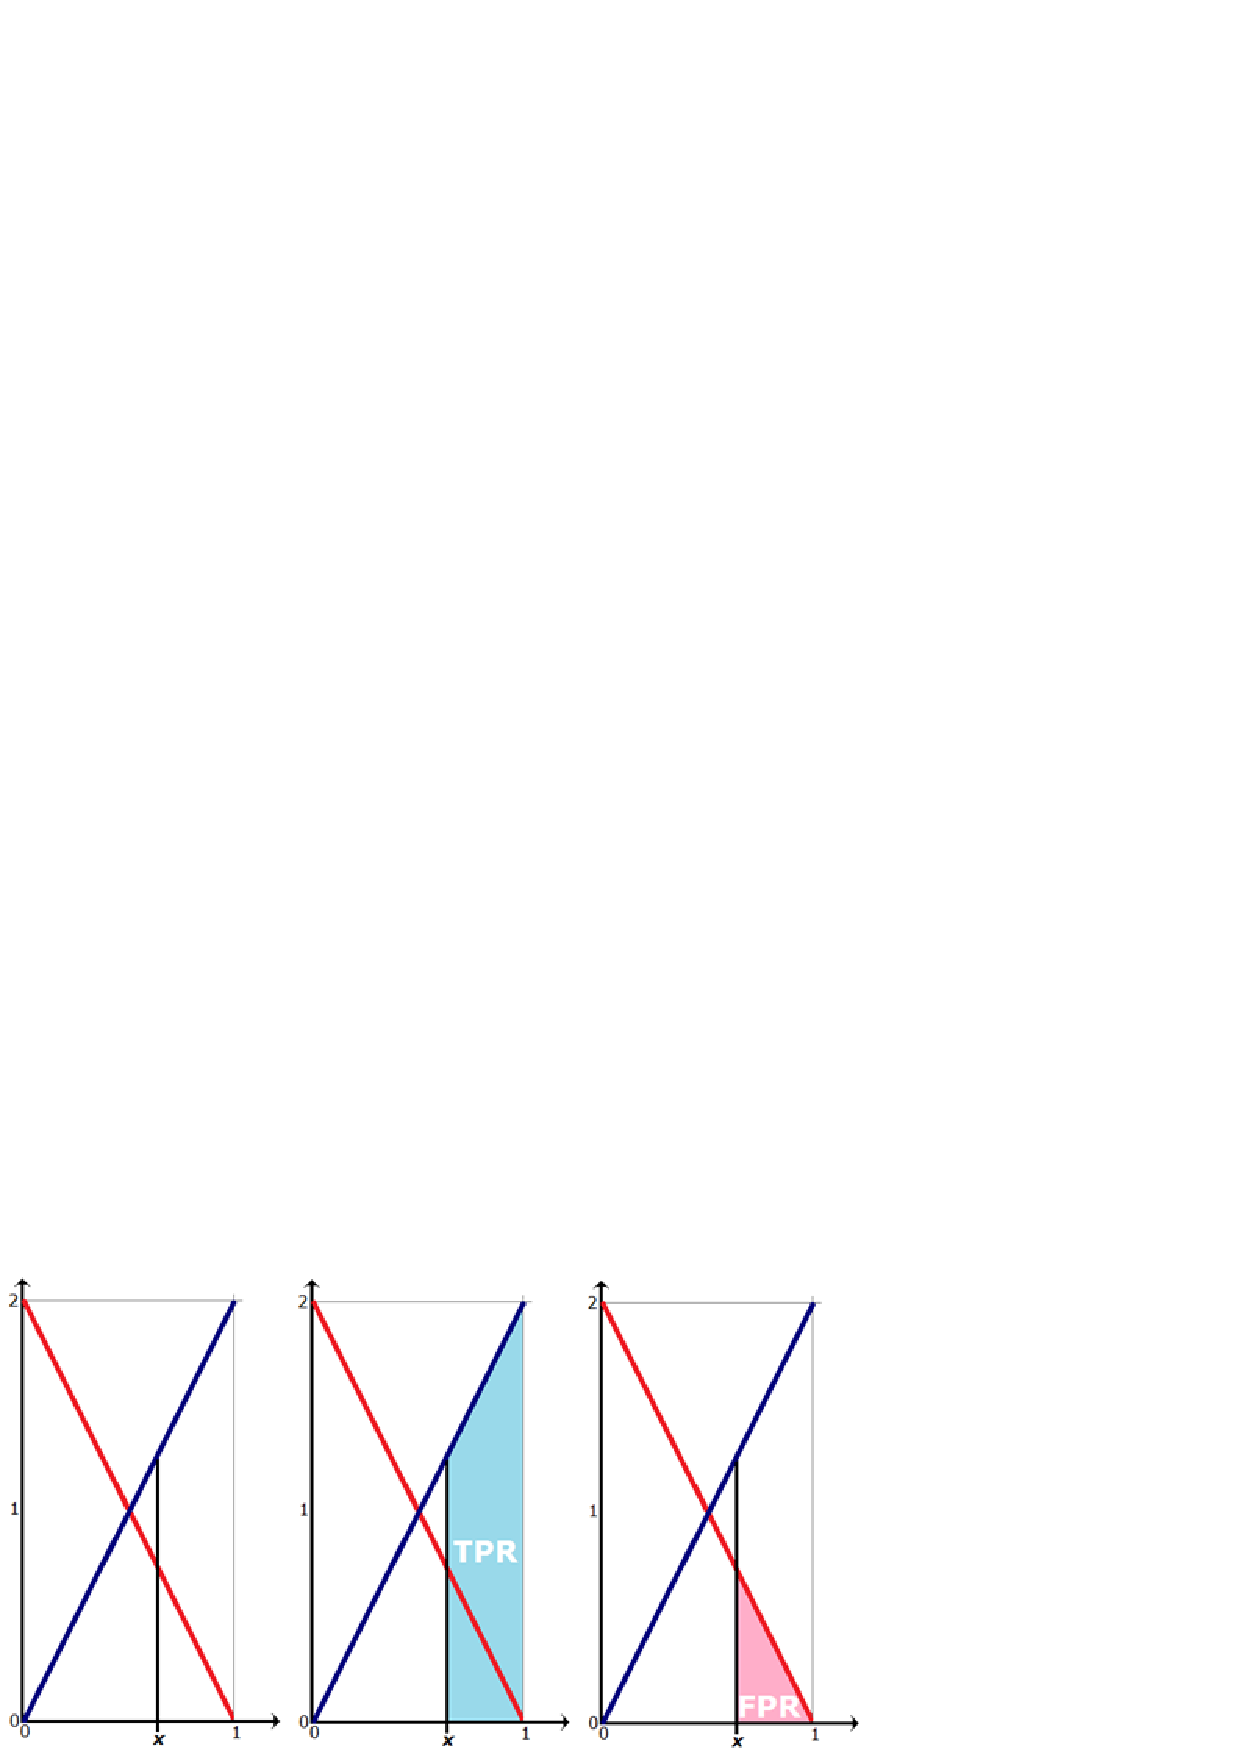
\includegraphics[width=0.5\textwidth]{./images/pic6.png}
	\caption{Распределение объектов положительного и отрицательного классов}
 \label{fig:densities}
\end{figure}

\begin{esSolution}
Для выбранного порога бинаризации $t$ значение TPR будет равно отношению площади трапеции, отсекаемой вертикальной прямой $y = t$ под синей прямой (см. рисунок) к площади всего треугольника под синей прямой.
Площадь под синей прямой равна единице (во-первых, по условию синяя прямая задаёт плотность, во-вторых, можно проверить вручную).
Площадь трапеции можно выразить как разность площадей треугольников: $TPR(t) = 1 - \frac{t \cdot 2t}{2} = 1 - t^2.$
Для FPR идея аналогичная, но нужно посчитать площадь треугольника, а не трапеции: $FPR(t) = \frac{1}{2}(1 - t)(2 - 2t) = (1 - t)^2.$
Теперь можно выразить TPR через FPR:
$TPR(t) = 1 - (1 - \sqrt{FPR(t)})^2 = 2\sqrt{FPR(t)} - FPR(t).$
Значит, ROC-кривая задаётся уравнением $y = 2\sqrt{x} - x.$
Площадь под ней можно посчитать, взяв следующий интеграл:
$$
\int\limits_0^1 (2\sqrt{x} - x)dx = \left(\frac{4}{3}x^{\frac{3}{2}} - \frac{1}{2}x^2\right)\bigg|_0^1 = \frac{5}{6}.
$$

\textbf{Задача 1.5.}
У банка всего 4000 клиентов. Маркетингового бюджета нового пред-
ложения банка хватит на то, чтобы обзвонить 800 клиентов. По историческим дан-
ным аналитики банка выяснили, что лишь 6 \% клиентов действительно начинают
пользоваться новым предложением после маркетингового звонка. У компании уже
есть два классификатора A и B, для которых положительный класс – это клиен-
ты, которые отреагируют на маркетинговый звонок, а отрицательный – клиенты,
на которых он не повлияет. Известно, что для A FPR = 0.1, TPR = 0.2, а для B
FPR = 0.25, TPR = 0.6. Постройте на их основе классификатор, который выберет
ровно 800 клиентов для совершения маркетинговых звонков. \\

\begin{esSolution}
Запишем условие на то, что классификатор выберет ровно 800 клиентов: $FPR \cdot \ell_{-} + TPR \cdot \ell_{+} = 800.$
Это можно представить в виде прямой, заданной в том же пространстве, что и ROC-кривая.
Чему равны $\ell_{-}$ и $\ell_{+}$ в нашем случае?
Воспользуемся данными аналитиков и получим, что среди всех клиентов будет $0.06 \cdot 4000 = 240$ клиентов, относящихся к положительному классу, и 3760 клиентов, относящихся к отрицательному классу.

Посмотрим, сколько объектов положительного класса нам выдадут классификаторы $A$ и $B$.
Для $A$: $0.1 \cdot 3760 + 0.2 \cdot 240 = 424$ -- слишком мало
Для $B$: $0.25 \cdot 3760 + 0.6 \cdot 240 = 1084$ -- слишком много.

Проведём отрезок между точками $A$ и $B$ в пространстве ROC-кривой.
Заметим, что мы можем получить любой классификатор с парой характеристик $(FPR, TPR),$ лежащей на этом отрезке.
Для этого нам достаточно брать предсказания данных двух классификаторов с вероятностями, пропорциональными расстояниям от точки до концов отрезков.

Выпишем уравнение прямой, проходящей через точки $A$ и $B$, и найдём её точку пересечения с прямой, заданной в условии.
Для прямой, проходящей через точки $A$ и $B$ верно, что 
$$
\begin{cases}
    0.2 = a \cdot 0.1 + b\\
    0.6 = a \cdot 0.25 + b
\end{cases}
\Leftrightarrow 
\begin{cases}
    b = 0.2 - a \cdot 0.1\\
    0.4 = a \cdot 0.15
\end{cases}\Leftrightarrow \begin{cases}
    a = \frac{8}{3}\\
    b = -\frac{1}{15}
\end{cases}.
$$
Значит, нам надо найти точку пересечения прямых $TPR = \frac{8}{3} \cdot FPR - \frac{1}{15}$ и $TPR = \frac{10}{3} - \frac{47}{3} \cdot FPR.$ Получаем точку $FPR = \frac{51}{275}, TPR = \frac{353}{825}.$
Осталось посчитать отношение, в котором эта точка делит отрезок:
$$\frac{\frac{51}{275} - \frac{1}{10}}{\frac{1}{4} - \frac{1}{10}} = \frac{94}{165}.$$
Значит, для получения искомого классификатора с вероятностью $\frac{94}{165} \approx 0.57$ надо брать предсказание классификатора $B$, иначе -- предсказание классификатора $A$.
Иллюстрацию к задаче можно найти на рис. \ref{fig:const}.

\begin{figure}[th!]
	\centering
	\includegraphics[width=0.4\textwidth]{./images/ml_roc_cross.png}
	\caption{Иллюстрация к задаче 1.5}
 \label{fig:const}
\end{figure}

\newpage
\textbf{Задача 1.6.}
Зафиксируем число объектов положительного $l_{+}$ и отрицательного
$l_{-} $классов. Докажите, что ROC-кривая классификатора A не ниже ROC-кривой
классификатора B в любой точке тогда и только тогда, когда PR-кривая классифи-
катора A не ниже PR-кривой классификатора B в любой точке. \\

\begin{esSolution}
Докажем, что если ROC-кривая выше, то и PR-кривая выше.
Выберем для двух классификаторов такие пороги $t_1$ и $t_2$, что $TPR_A(t_1) = TPR_B(t_2).$
Проверим, как при этом соотносятся их точности.
Известно, что ROC-кривая $A$ выше ROC-кривой $B$, поэтому $FPR_A(t_1) \leqslant FPR_B(t_2) \Leftrightarrow FP_A(t_1) \leqslant FP_B(t_2).$
Вспомним формулу для точности: $PR_A(t) = \frac{TP_A(t)}{TP_A(t) + FP_A(t)}.$
Из условия $TPR_A(t_1) = TPR_B(t_2)$ следует равенство $TP_A(t_1) = TP_B(t_2),$ а значит, $PR_A(t_1)$ и $PR_B(t_2)$ отличаются только за счёт $FP$ в знаменателе.
Воспользовавшись полученным выше неравенством на $FP$, получаем, что $PR_A(t_1) \geqslant PR_B(t_2),$ ч.т.д.. 

Доказательство в обратную сторону проделывается абсолютно аналогично: надо зафиксировать пороги с равной полнотой и сравнить точности.
Как и в прошлом случае, точности будут отличаться только за счёт $FP$, так что из неравенства точностей мы получим неравенство для $FPR$. \\

\textbf{Задача 1.7. Обратимая ли PR-кривая?}
Рассмотрим бинарный классификатор, который каждой выборке из \( N \) объектов сопоставляет оценки 
\( b_i \in [0,1] \), \( i = 1, \dots, N \).  
Пусть истинные метки обозначены как \( y_i \in \{0,1\} \). Так же дополнительно известна $\pi$ - доля положительных примеров в выборке.

Пусть PR-кривая классификатора задана в аналитическом виде, то есть известна точная зависимость $Precision = $f$(Recall)$.

\begin{enumerate}
    \item Докажите, что зная функцию $f(Recall)$ и значение \(\pi\), можно восстановить ROC-кривую (то есть получить зависимость TPR от FPR).

    \item Найдите явное выражение для \( FPR \) через \( Precision \), \( Recall \) и \(\pi\).
\end{enumerate}

\textbf{Решение:}
Используя соотношения:
\[
Precision = \frac{TP}{TP + FP}, \quad Recall = \frac{TP}{TP + FN}, \quad \pi = \frac{TP + FN}{N}.
\]
Можно выразить через эти параметры \(FP\), \(FN\) и получить
\[
FPR = \frac{FP}{FP + TN},
\]
учитывая, что \( FP + TN = (1 - \pi)N \).

\textbf{Ответ.}
\[
FPR = \frac{\pi \, Recall \, (1 - Precision)}{(1 - \pi) \, Precision}, 
\qquad
TPR = Recall.
\]

\textbf{Комментарий.}
При известной PR-кривой \( Precision(Recall) \) и доле положительных \(\pi\),
ROC-кривая однозначно восстанавливается.
Однако без знания \(\pi\) обратное преобразование невозможно,
так как ROC-кривая инвариантна к изменению соотношения классов,
а PR-кривая --- нет.


\section*{Прямая оптимизация AUC-ROC}
При обучении модели в бинарной классификации чаще всего решается задача минимизации верхней оценки функционала ошибки:

$$
Q(a, X)=\frac{1}{\ell} \sum_{i=1}^{\ell}\left[a\left(x_{i}\right) \neq y_{i}\right] \leq \frac{1}{\ell} \sum_{i=1}^{\ell} \tilde{L}\left(M_{i}\right) \rightarrow \min _{w}
$$

Однако иногда возникает необходимость оптимизировать более сложные метрики - в частности, AUC-ROC. Напрямую оптимизировать подобные метрики не представляется возможным из-за их дискретной структуры, однако мы можем использовать трюк с верхней оценкой функционала ошибки и в этом случае. В задаче 1.1 мы показали, что AUC-ROC связан с долей дефектных пар в выборке, поэтому максимизация AUC-ROC равносильна минимизации доли дефектных пар.

$$
\begin{aligned}
& D P(b, X)=\frac{2}{\ell(\ell-1)} \sum_{i<j}^{\ell}\left[y_{i}<y_{j}\right]\left[b\left(x_{i}\right)>b\left(x_{j}\right)\right]= \\
& \frac{2}{\ell(\ell-1)} \sum_{i<j}^{\ell}\left[y_{i}<y_{j}\right]\left[b\left(x_{j}\right)-b\left(x_{i}\right)<0\right] \leq \frac{2}{\ell(\ell-1)} \sum_{i<j}^{\ell}\left[y_{i}<y_{j}\right] \tilde{L}\left(b\left(x_{j}\right)-b\left(x_{i}\right)\right) \rightarrow \min _{b}
\end{aligned}
$$

Если верхняя оценка $\tilde{L}$ дифференцируема по параметрам модели, то можно оптимизировать такой функционал при помощи градиентных методов.


\end{document}